\section{Barbarian Class Weapons}

\subsubsection{Strom'kar the Warbreaker}

Strom'kar the Warbreaker is an ancient weapon of legend. It is said to have been forged in the lava's underneath the rumored great city of Ironforge. To contain the energies that dance across its cold edges, Shadowmourne was believed to have been hewn from piles of impure Saronite and the hardened blood of the Old God, Yogg-Saron. The weapon is said to have been forged by a group of master blacksmiths and weapon artisans. The weapon was wielded by the Dwarven kings in the times when Ironforge was at its prime. It is said that this weapon was used particularly by a great king Gimly Branbeard whom used the weapon to slay an enchanted ice dragon that was mind controlled and sent onto the city of Ironforge by the Lich King. Rumor has it that this weapon was buried with the King as it's power became too great for anyone to wield. The weapon in the legends is believed to have absorbed the essence of the ice dragon after its defeat.

\begin{center}
	
\includegraphics[width=\linewidth]{img/weapons/stromkar.jpg}
\end{center}

\subsubsection{Potential}

Strom'kar the Warbreaker weapon wants to be wielded by a righteous Barbarian. 

\begin{commentbox}{Strom'kar the Warbreaker\footnote{Weapon (greataxe), artifact (requires attunement by a barbarian)}}	
	You gain a +3 bonus to attack and damage rolls made with this magic weapon. When you hit an enemy you will deal 2d6 slashing damage and 2d6 thunder damage. The damage will change to d10's if the target has less than 15 strength.
	
	While a Barbarian wields The Strom'kar in combat it will look like the Barbarian is glowing with a light gray aura. Any physical attack taken while wielding this weapon will have it's damage reduced by 2d6 damage.
	
	If a Barbarian of an evil alignment tries to attune to The Strom'kar they have to make a d20 roll. At a 18 or below The Strom'kar will reject you and deal 6d10 thunderous damage. At a 19 or 20 you over power the will of the weapon and make it yours.
	
	With a successful roll to overcome the will of The Strom'kar while having an evil alignment will make The Strom'kar appearance will start to dull and become darker until it becomes fully corrupt. It will regain its former glory when its attuned to a paladin of a non evil alignment.
	
	Proficiency with a greataxe allows you to add your proficiency bonus to the attack roll for any attack you make with it.
	
	If the wielder of Strom'kar dies (by failing three death saves) then the life essence of the blade can leave the weapon and resurrect the player to full. The weapon after this point will shatter and become useless. The essence from the Dragon within the blade will transfer to the wielder.
\end{commentbox}

\subsubsection{Finding Strom'kar the Warbreaker}

When not being wielded, Strom'kar is overpowered by the essence of Yogg-Saron whose blood helped forge it's edge. Yogg-Saron's influence over the blade seeks to cause insanity among those who would dare approach the blade. The blade in this state seeks to consume all. Strom'kar resides in a dark cave with the entrance being a large opening in the grass of a dense region of forest. Upon entering the cave, anyone would begin to become insane. The closer they get to the blade, the further the insanity is driven. The only way to stop the insanity from ensuing is to find and wield the blade and overcome it if worthy. This can only be done by a righteous barbarian. 

\begin{commentbox}{Insanity of Yogg-Saron from Strom'kar}
	Insanity can be seen as a 5 stage process. Fear leads to anger, anger leads to hate, hate leads to suffering, and suffering leads to death. When under the influence of Yogg-Saron, one can hear and see images and visions from Yogg-Saron as well as take damage that is either self inflicted or psychic damage.
	\begin{itemize}
		\item Level 1 Insanity: Fear. The first step in reaching insanity is an immense fear ensued within the victims. 
		\item Level 2 Insanity: Anger. From the fear, the victims will become angry and chaotic wanting to escape their current state but unable to.
		\item Level 3 Insanity: Hate. From the anger they are wielding, they will begin to hate those around them and those who got them into the situation they are in.
		\item Level 4 Insanity: Suffering. From their hatred the players will begin to suffer as they have approached the peak of insanity.
		\item Level 5 Insanity: If the players stay in the suffering phase of insanity, they will die by driving their mental state to a point where they do not want to live and commit suicide in a slow and painful way.
	\end{itemize}

\begin{center}
	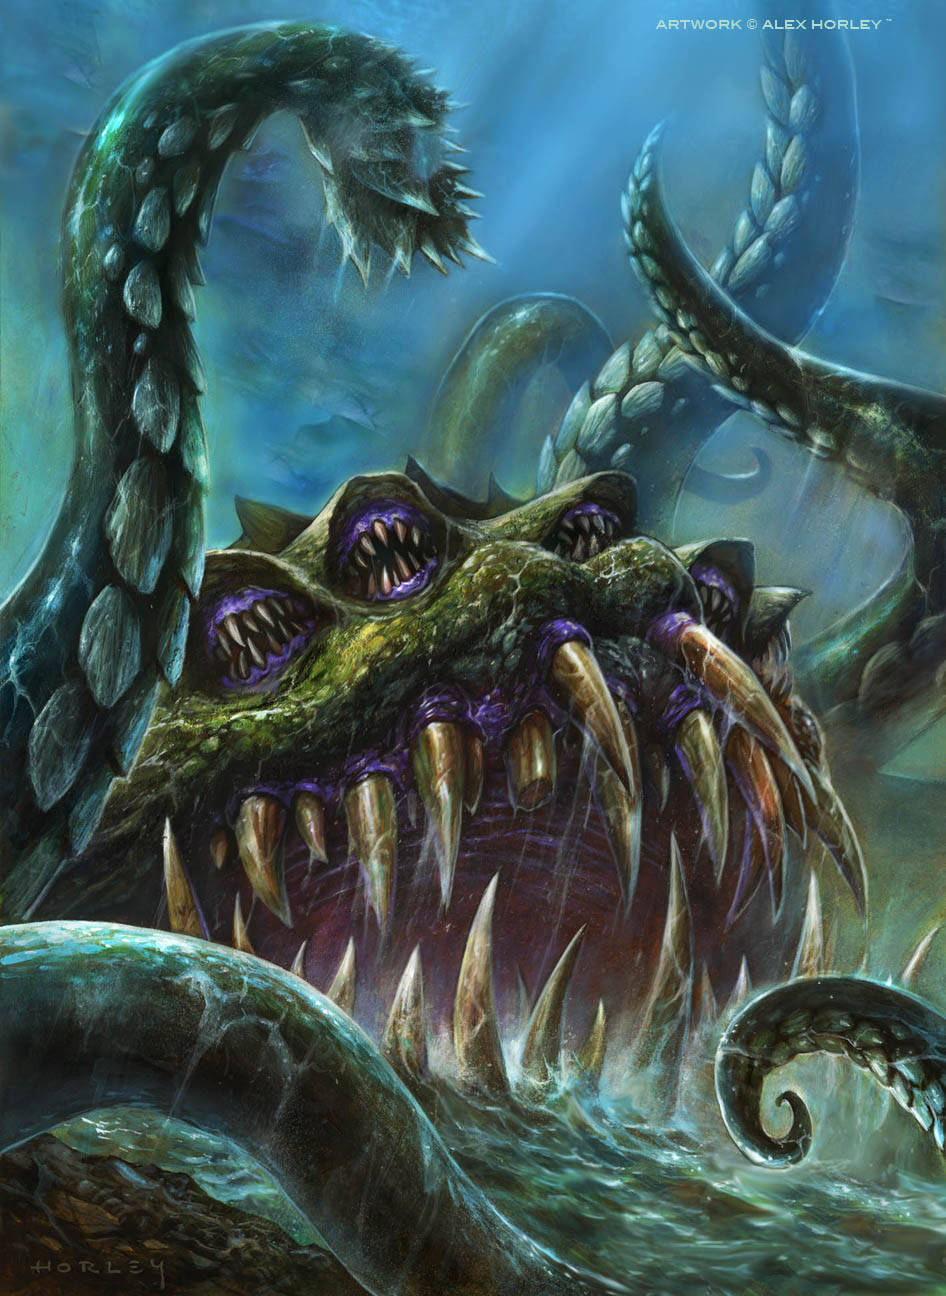
\includegraphics[width=0.4\linewidth]{img/WoW/CallofYogg-Saron.jpg} 	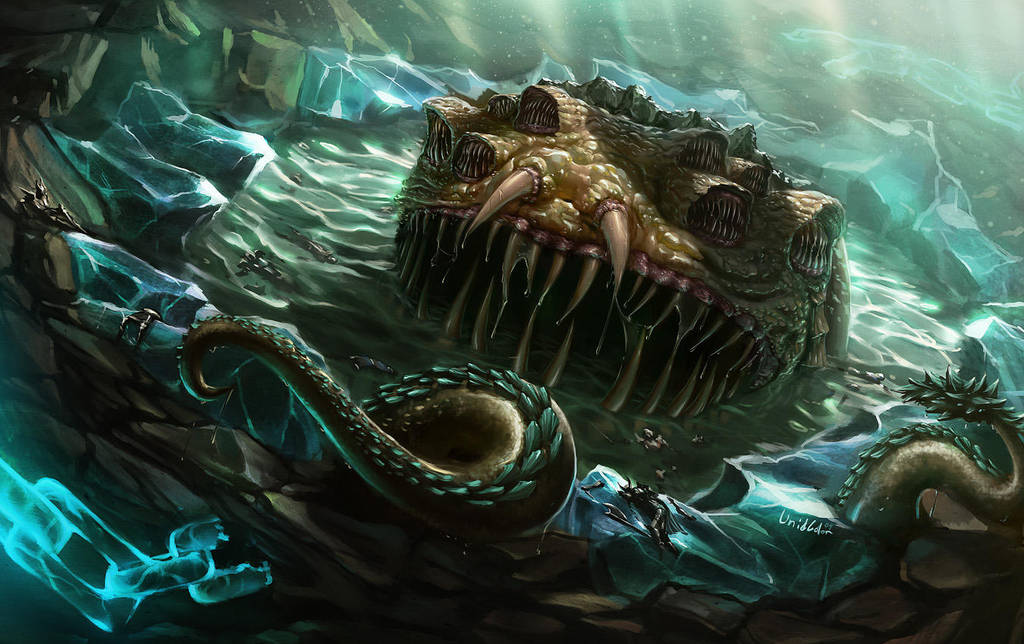
\includegraphics[width=0.59\linewidth]{img/WoW/yoggsarond210alw-fullview.jpg}
\end{center}
\end{commentbox}

Strom'kar is inherently a blade of righteous character and power. Even when overcome by the power of Yogg-Saron, it still has some ability to act on it's own. This ability is normally not capable of overpowering the influence of Yogg-Saron, however when nearby victims have reached level 3 or 4 insanity, the blade can overpower it's dark influence and show its hidden self to the victims. This gives them a chance to wield the blade if they so take the leap. During this point, if the wielder is worthy, they will have the opportunity to put away the influence of Yogg-Saron within the blade and end the insanity they are enduring. However, if the wielder is not able to wield Strom'kar, then there is none other fate that that of Yogg-Saron's insanity.